\documentclass[10pt,a4paper]{article}
\usepackage{inputenc}
\usepackage[english]{babel}
\usepackage[T1]{fontenc}
\usepackage{amsmath}
\usepackage{amsfonts}
\usepackage{amssymb}
\usepackage{graphicx}
\usepackage{epstopdf}
\usepackage{url}
\usepackage{algorithm}
\usepackage{algpseudocode}
\usepackage{algorithmicx}
\usepackage{tikz}


%\floatname{algorithm}{Procedure}
\renewcommand{\algorithmicrequire}{\textbf{Input:}}
\renewcommand{\algorithmicensure}{\textbf{Output:}}

\addtolength{\hoffset}{-1.5cm}
\addtolength{\textwidth}{3.5cm}

\title{Top-Down and Bottom-up Cues for Scene Text Recognition, \\
A. Mishra, K. Alahari, C. V. Jawahar}
\author{Vincent BODIN \& Thomas MOREAU}
\date{}


\begin{document}
\maketitle

\hrulefill
\begin{abstract}
\emph{Scene text recognition refers to finding automatic ways of extracting text in pictures of everyday life. As computer vision is more and more successful, scene text recognition has naturally become a significant issue nowadays. Unlike OCR which is more or less well understood and implemented, scene text recognition still needs many improvements to be considered as a powerful tool. We implemented a paper \cite{Mis} that explains how to extract words efficiently. A graphical model is introduced inside, with the creation of graph representing possible detected words. The algorithm TRW-S \cite{Kol}, which is a slightly different version of Belief Propagation (BP) is used to extract the optimal words.}
\end{abstract}






%\newpage
%\tableofcontents
%\newpage



\section*{Introduction}

Understanding scenes semantically has gained considerable consideration for those last few years with the successes of computer vision. In particular, a certain attention has been granted to street scenes, whether it takes the form of object detection, object recognition or segmentation. We decided to consider a slightly different problem, though the methods may be quite similar. We decided to focus on text recognition in streets. It is indeed a project that has potentially considerable repercussions in our everyday life. \\

For this, we decided to implement a paper \cite{Mis} that details a method to retrieve in natural pictures some characters and interpret it as words. Their results seem to be the highest reached till now in this field of computer vision and it includes some graphical models and algorithm for minimizing a discrete energy on a graph (TRW-S, \cite{Kol}). It mainly requires two steps:
\begin{description}
\item[Step 1:] Detect all the possible characters in the picture. We should be very exhaustive in here, we do not want to miss any character because that would basically hamper us from retrieving any word. This character detection is possible through machine learning methods. We learn $K$ SVMs - one-versus-all method and we learn one SVM for each character - and then we scan the image and test for each patch whether there can potentially be a character or not.

\item[Step 2:] Among all those possible characters, we try to prune and reconstruct words. From all the sliding windows remaining after this process, we build a graph that takes its value in $\mathcal{K}_{\epsilon}$ the set of all characters plus a void label to discard the false positives. We then assign an energy on this graph depending on unary energies of each nodes and pairwise energies. Then we will run an algorithm to extract a lower bound of the energy minimization problem - which is NP-hard. 
\end{description}
In this project we will essentially be interested in the first step of the project, the second one being implemented in \emph{Probabilistic Graphical Model} course.






\section{Learning preliminaries}

\subsection{Learning characters}

The first task we have to deal with is extracting characters from a natural image. This is done through a specific classifier learned on some database of characters. We used the databases ICDAR 2003 \cite{ICDARchar} and Chars74K \cite{Char74K} for training our SVM. From each patch of character, we resize it to a $22\times 20$ window from which we extract a Histogram Of Gradient (HOG) \cite{Dal2005}: this is the feature vector we are working with. We kept 12 directions in the HOG, because it empirically seemed to give the best results. \\

We then need to train our classifier, this is done through a one-versus-all procedure. It yields to $K = |\mathcal{K}|$ classifiers where $\mathcal{K}$ is the set of all possible character. As we deal with the English language, the cardinality of $\mathcal{K}$ is equal to 62. The SVM are trained with a Kernel, the so-called RBF kernel $\exp(-\gamma |x-x'|^2), \gamma > 0$. It allows to distord the euclidean metric to catch local changes. We used a Python library scikit-learn \cite{scikit}. The issue with this method is the number of parameters we have to deal with: $K$ coefficients $\gamma$ and regularization $C$ - one for each classifier. We performed an exponential grid-search cross-validation to find the 'almost' optimal values of those coefficients. Yet, the test error only fell by $10\%$ doing so: from a $25\%$ error on the training set with naive coefficients to $16\%$ with tuned parameters. We will talk again about this later on. 


\subsection{Learning words}

The second task for the learning process is to build a lexicon prior, \emph{i.e.} learning how letters interact to create words. The whole idea of this step is to be able to determine among a large number of words possibilities which on is the most likely to be indeed written. The database used was ICDAR 2003 word \cite{ICDARword}. Then we used the bi-gram method which consists in learning how pairs of letters interact together. This is done via a counting of occurrences of each pair $(c_i,c_j)$ to determine though its empirical frequency the probability $p(c_i,c_j)$. This probability will be re-used afterward in an energy term penalizing the pairs that might not occur frequently. 




\section{Character detection}

Given what we have learned, we now deal with character detection in an actual natural image. This is done via a sliding window scanning, as explained in \ref{algo1}. The idea is to scan the image with different aspect ratio patches, denoted by $a_i$ for the scanning window $l_i$. Then we use our $K$ classifiers to determine for each character if this patch might contain this character or not. A goodness score is attributed according to the following formula:
\begin{equation}
GS(l_i) = \max_c p(c|\phi_i) \exp\left( - \frac{(a_i - \mu_{a_j})^2}{2\sigma_{a_j}^2} \right)
\label{eq:}
\end{equation}
This GS is made of two parts: the first one is meant to determine is there is a probability that a character is in this patch, this is why we take the maximum of the probability of characters. This need nonetheless to be penalized by the aspect ratio learned from the database: if a $l$ is found in a window with a large width an small height, we might not want to keep it since it might not be a real $l$. \\

\begin{algorithm}
\caption{Sliding Window scanning}
\label{algo1}
\begin{algorithmic}
\Require Image
\Ensure l list of characters

\State l = [ ]; 
\For {all windows in Image}
	\State $p \leftarrow$ svm.predict\_proba
	\State GS $\leftarrow \max_c p(c|\phi_i) \exp\left( - \frac{(a_i - \mu_{a_j})^2}{2\sigma_{a_j}^2} \right)$
		\If {GS > 0.1}
		\State l.append(window) 
	\EndIf
\EndFor
\end{algorithmic}
\end{algorithm}

Having all those windows, many of them may represent the same character and we need to merge them. This is done by a specific Non-Maximum Suppression (NMS) for each character, given in \ref{algo2}. Note that the NMS algorithm we use here is character specific.

\begin{algorithm}
\caption{Non-Maximum Suppresion (NMS)}
\label{algo2}
\begin{algorithmic}
\Require $l$ list of windows, $c$ character with maximum probability for each window, threshold
\Ensure $l_p$ pruned list

\While {$l$ is not empty}
	\State $w_1, c_1$ pair of characters in l with highest probability
	\State $m = [w]$
	\For {$w_2,c_2$ in $l,c$}
		\If {criterion > threshold and $c_1 == c_2$}
			m.append($w_2$)
		\EndIf
	\EndFor
	\State $l_p$.append(mean($m$),$p$)
\EndWhile
\end{algorithmic}
\end{algorithm}



\section{Recognizing words}

Given the $n$ remaining windows we build a graphical model that will contain the underlying information of how related the letters are in our image. The key idea is that two letters apart should not be close in the reconstruction of a word and might not even have any influence one on another. First we should ensure that we reorganize our data in a lexicographic way so that we only put links between a node and the one that are very close to it as we will see above. This is the main pre-processing needed. 
\begin{description}
\item[Step 1: ] For each sliding window kept, assign a random variable $X_i$ that takes labels $x_i \in \mathcal{K}_{\epsilon}$ (add $\epsilon$ a void label).
\item[Step 2: ] When two sliding windows are 'close enough' build an edge between the nodes.
\item[Step 3: ] Assign CRF energy.
\end{description}

The energy is specified as a unary energy that penalizes a single character and a pairwise energy that takes into account how the letters interact to ceate words. The unary energy is: 
\begin{equation}
\begin{array}{rll}
E_i(x_i = c_j) & = & \displaystyle 1 - p(c_j|x_i) \\
E_i(x_i = \epsilon)	& = & \displaystyle \max_j p(c_j |x_i) \exp\left( - \frac{(\mu_{a_j} - a_i)^2}{2\sigma^2_{a_j}} \right)
\end{array}
\label{eq:}
\end{equation}
As for the pairwise energy, they should penalize pairs of letters that do not occur often in the lexicon, the form is the following:
\begin{equation}
\begin{array}{rlll}
E_{i,j}(x_i = c_i,x_j = c_j) 			& = & \displaystyle E^l(x_i,x_j) - \lambda_0\exp\left( - \psi(x_i,x_j) \right) 	& (\forall c_i \neq \epsilon, c_j \neq \epsilon) \\
E_{i,j}(x_i = c_i,x_j = \epsilon) & = & \displaystyle \lambda_0\exp\left( - \psi(x_i,x_j) \right) 								& \\
E_{i,j}(\epsilon, \epsilon) 			& = & \displaystyle 0 																													& \\
\psi_(x_i,x_j) 										& = & \displaystyle (100 - \text{overlap}(x_i,x_j))^2 													& \\
E^l(x_i = c_i,x_j = c_j)					& = & \displaystyle \lambda_l(1 - p(c_i,c_j)) 																	& (\text{lexicon prior})
\end{array}
\label{eq:pairwiseEnergy}
\end{equation}
So that we eventually obtain an energy on the graph $E:\mathcal{K}_{\epsilon}^n \rightarrow \mathbb{R}$ of the form:
\begin{equation}
E(\mathbf{x})	= \sum_{i=1}^n E_i(x_i) + \sum_{\mathcal{E} \text{ edges}} E_{i,j}(x_i,x_j)
\label{eq:}
\end{equation}
Hence we are led to minimizing the energy over the graph. This is a NP-hard problem and we will use an algorithm that provides an approximation: TRWS-S algorithm. We do not detail it here since it is the subject we dealt with in PGM course.





\section{Implementation and Results}

The implementation has been done with python2.7. The SVM part uses the implementation of the library \textbf{scikit-learn}. We have used the implementation of TRW-S of the libraries\textbf{Opengm} and \textbf{TRW-S.1-3} you can find on the web. To tune the SVM parameters, we have used a per-character grid-search over the parameters of regularization $C$ and the scale of our RBF kernel $\gamma$. This allows us to gain a character detection of $10\%$ while testing on our training set. We use a simple process to test our implementation. We started with the simplest case of OCR, with a printed word on a white background, already localized. We then used harder images as our results got better.

\begin{figure}[ht!c]
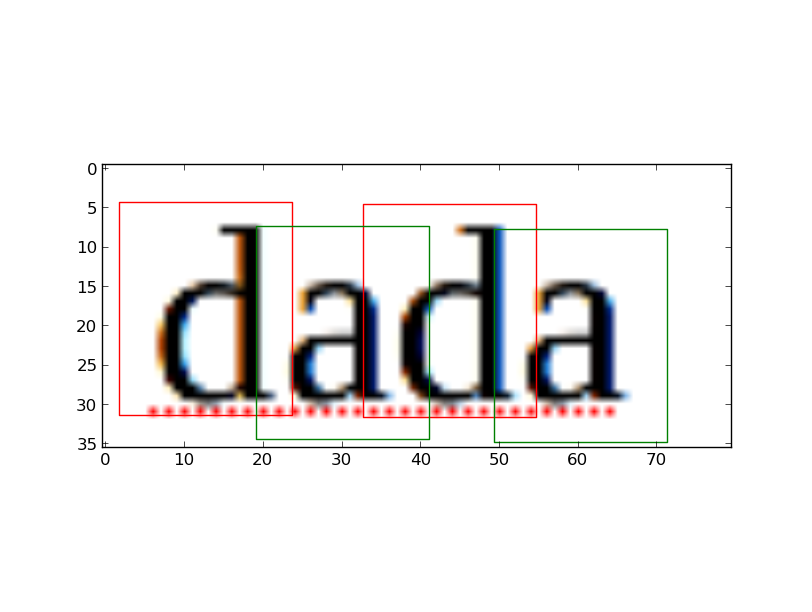
\includegraphics[width=0.3\columnwidth]{figures/dada1.png}
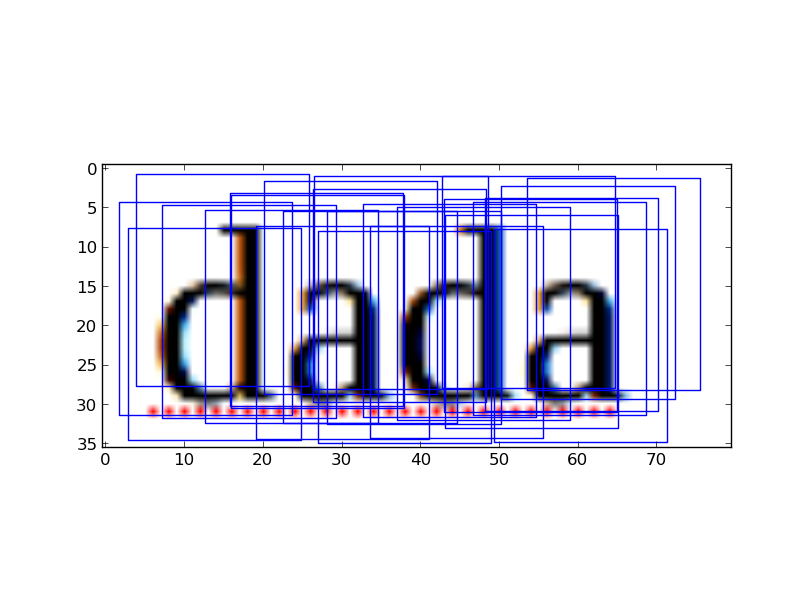
\includegraphics[width=0.3\columnwidth]{figures/dada2.png}%
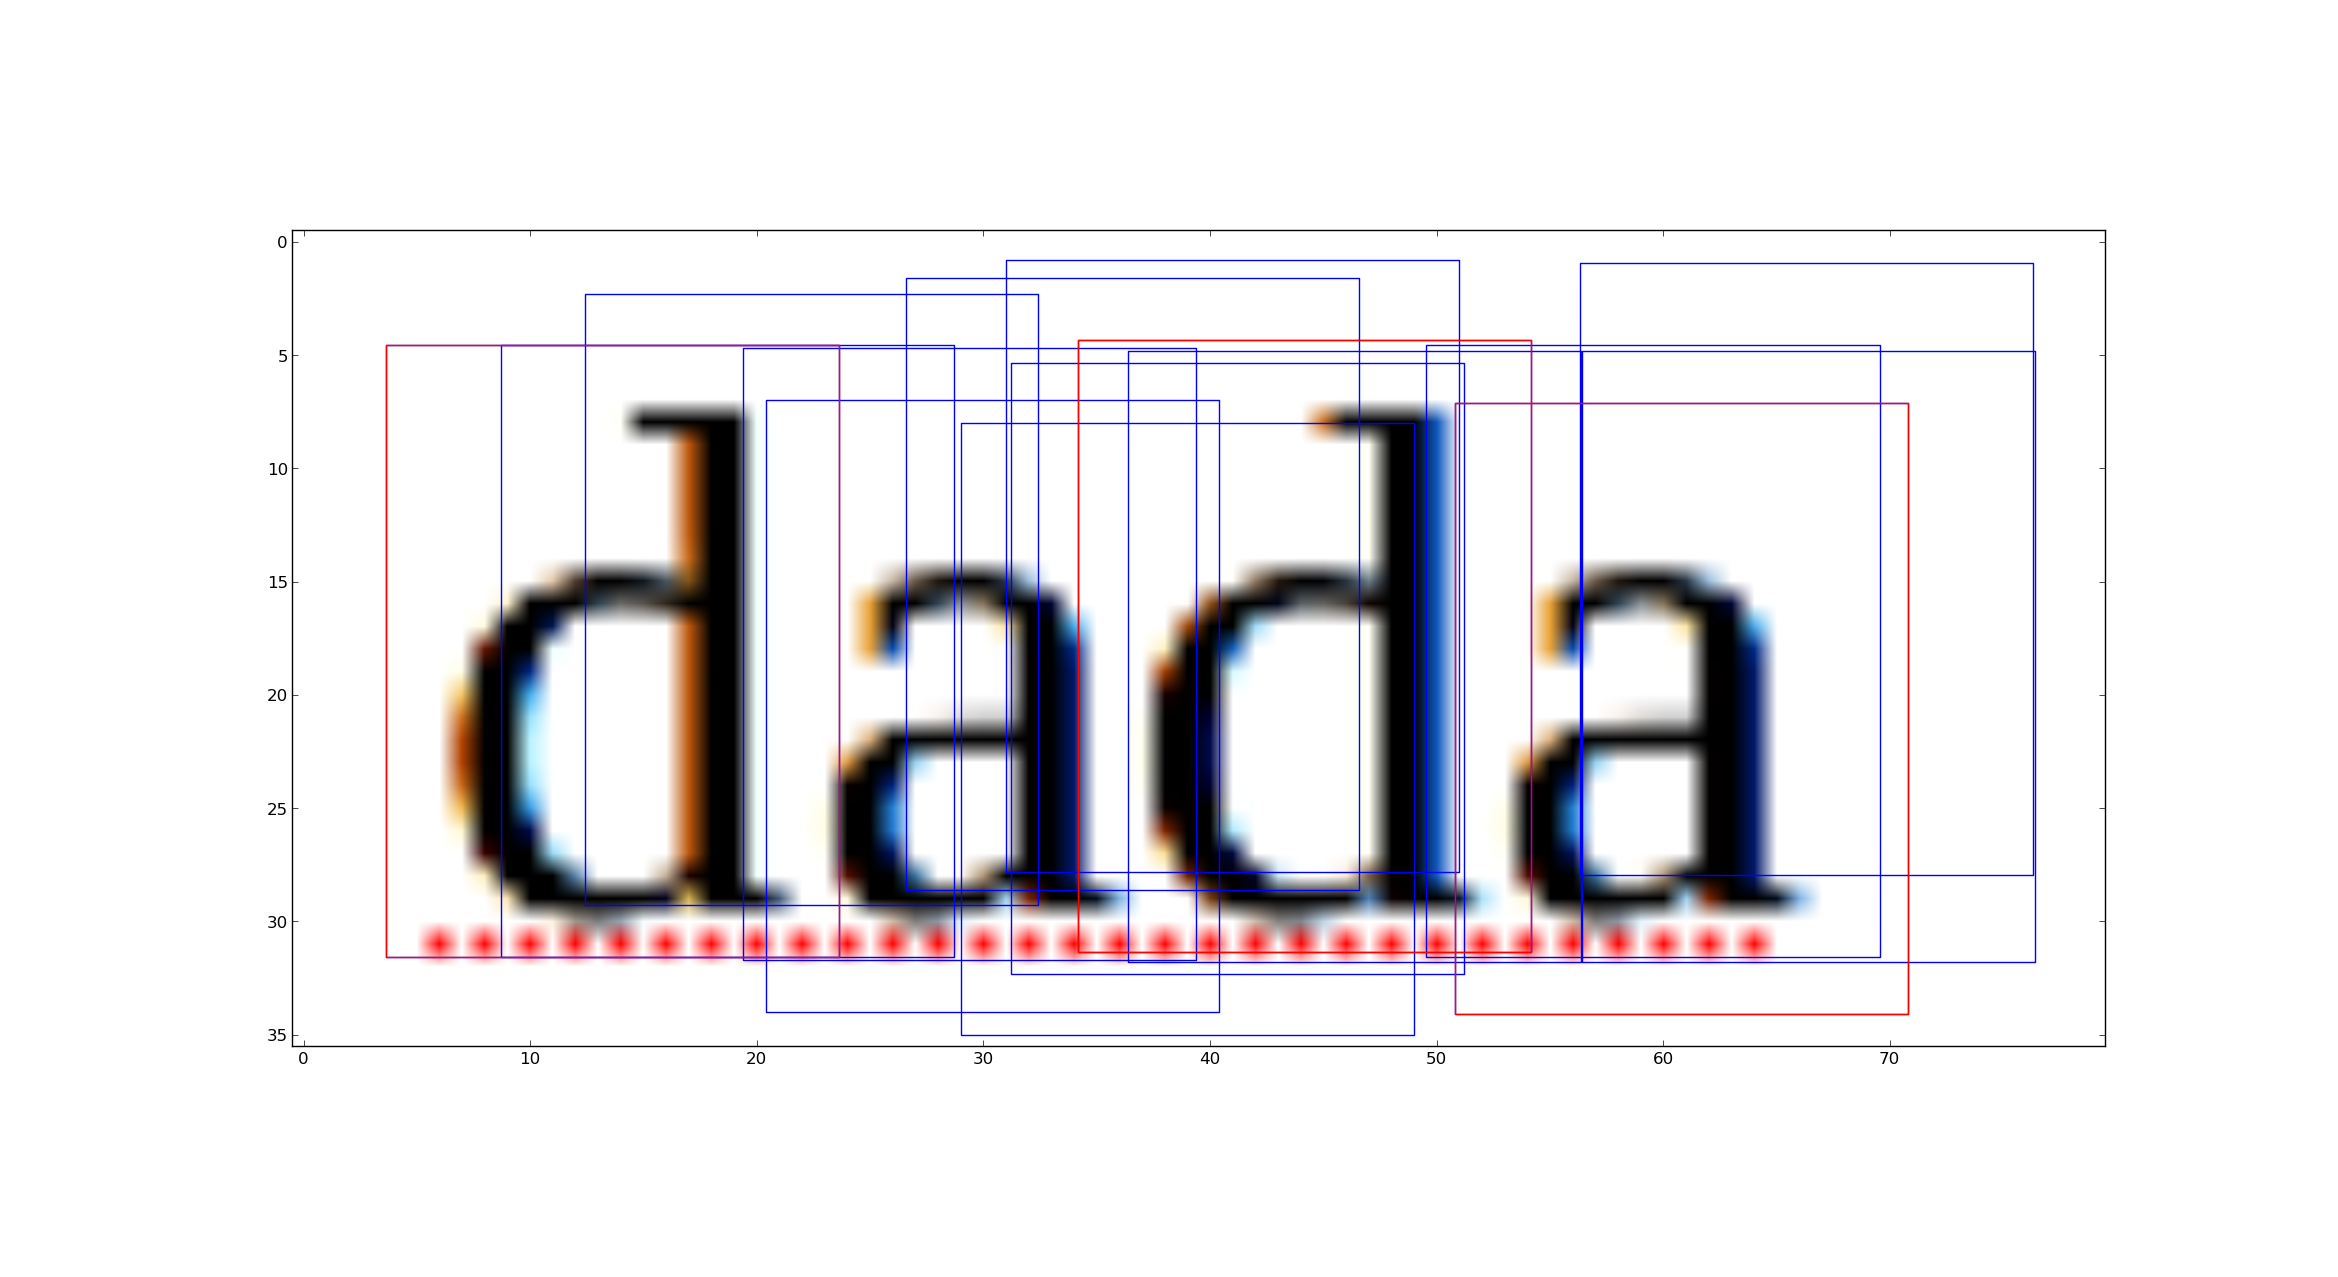
\includegraphics[width=0.3\columnwidth]{figures/dada3.png}%
\caption{Test on an artificial word 'dada'. Word retrieved: 'dda' or 'dd depending on the lexicon prior used}
\label{dada}
\vspace{0.5cm}
\centering
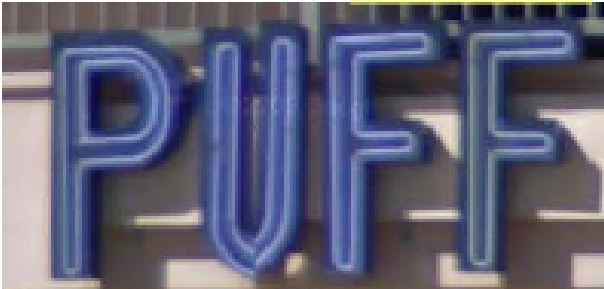
\includegraphics[width=0.4\columnwidth]{figures/puffTest.png}
\hspace{0.3cm}
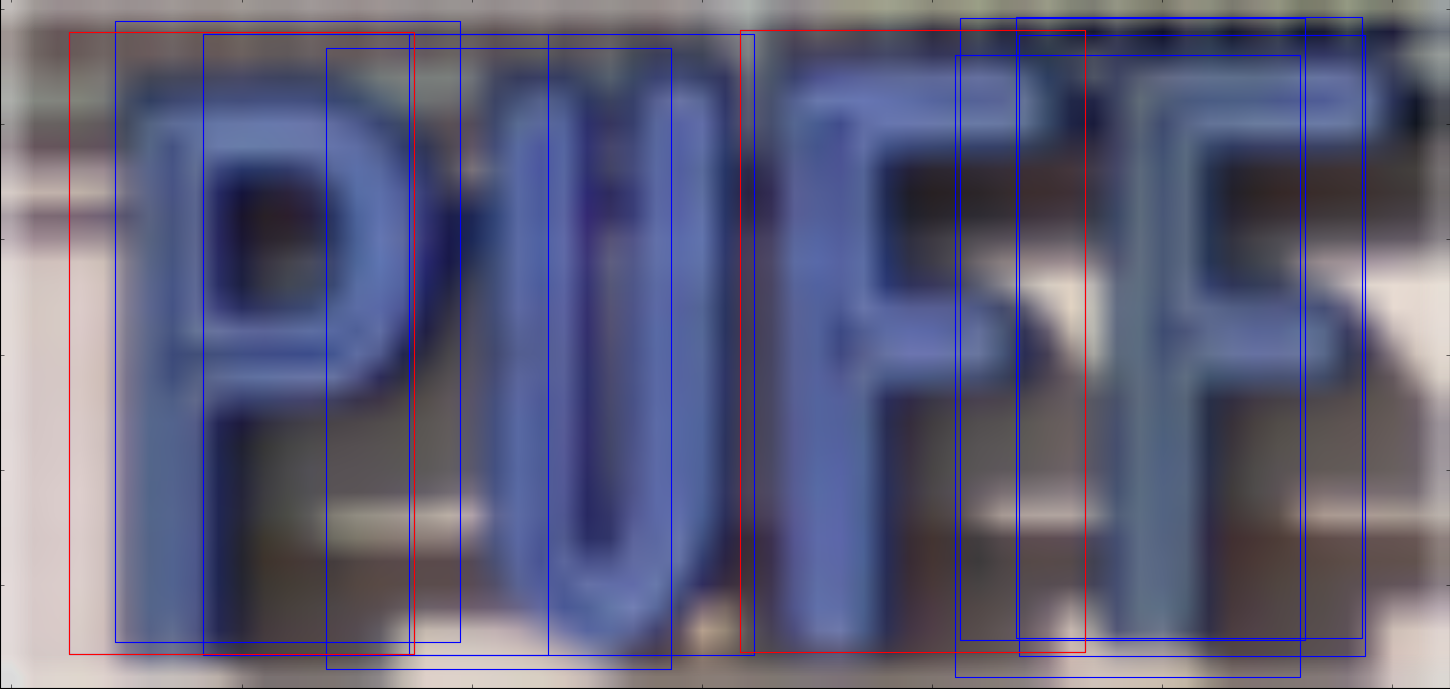
\includegraphics[width=0.4\columnwidth]{figures/puff.png}%
\caption{Natural testing word. Word retrieved: 'PE'}%
\label{Puff}
\vspace{0.5cm}
\centering
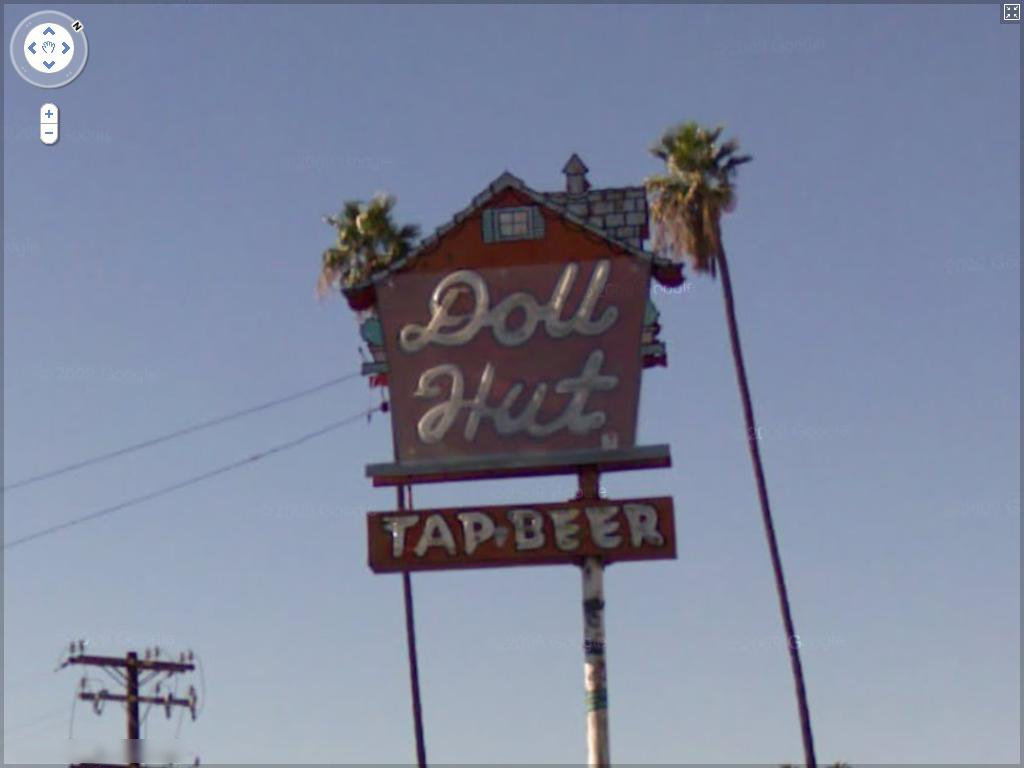
\includegraphics[width=6cm]{figures/00_00.jpg}
\hspace{0.3cm}
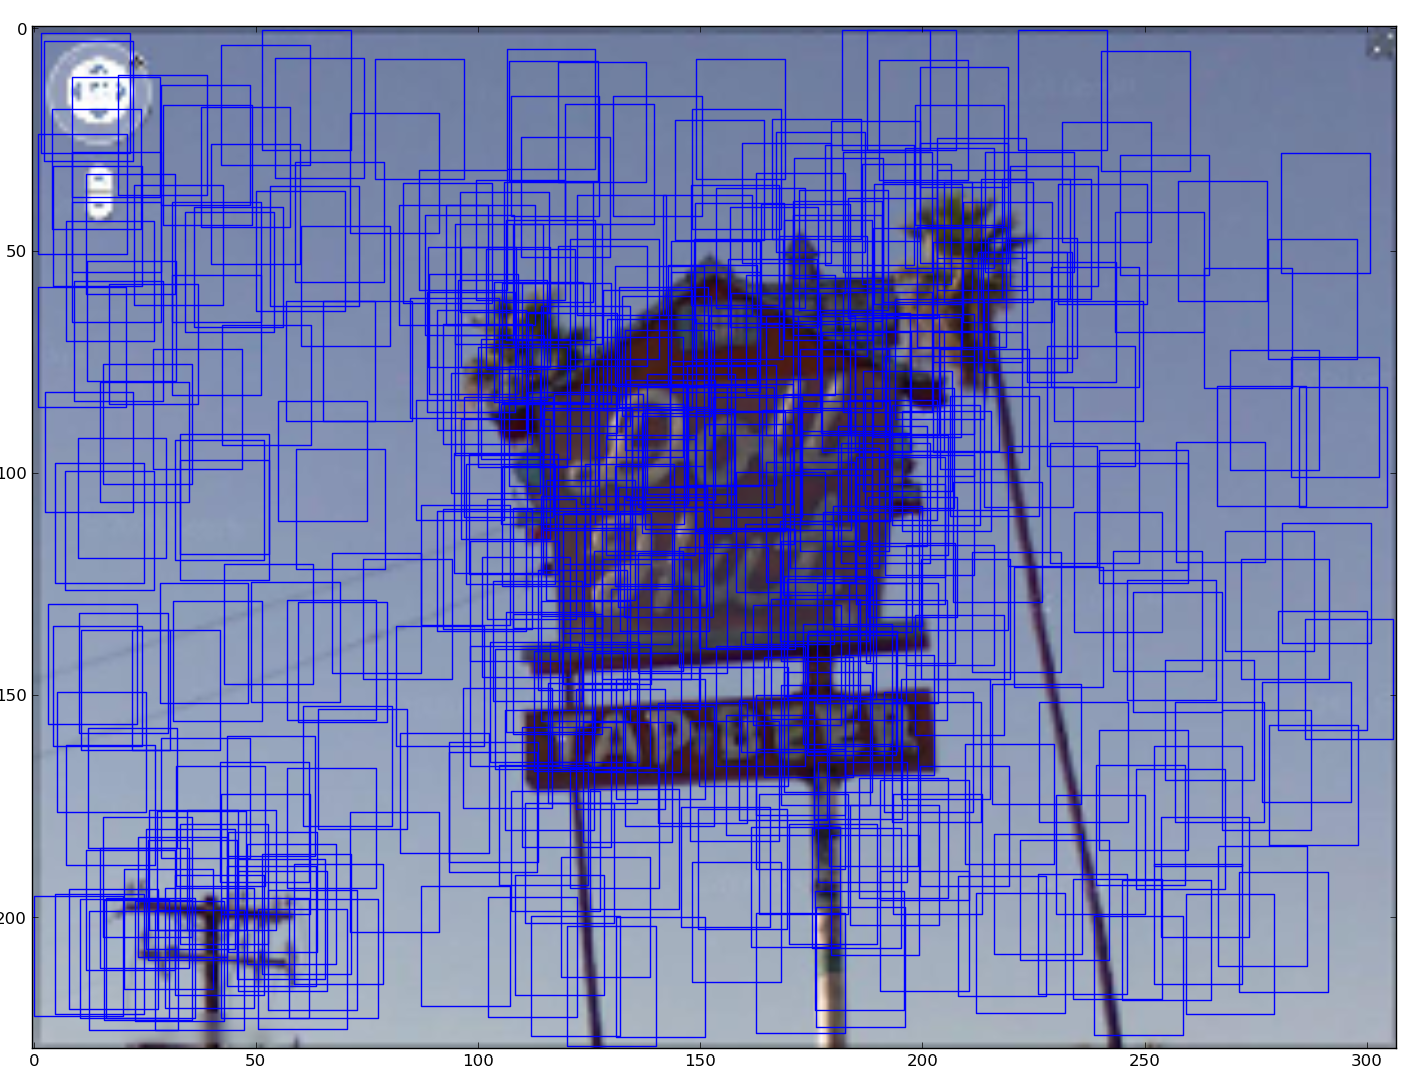
\includegraphics[width=6cm]{figures/beerResized.png}%
\caption{Natural testing image}%
\label{beer}
\end{figure}

We can see in the Fig.(\ref{dada}) that most of the time there are way too many characters that are detected but we are 'practically' able to select the correct ones with the graphical model. In the Fig.(\ref{Puff}), we can see two problems. The first one is the F is detected as a E by our SVM because of shadow perhaps. Then, the graphical model penalizes the overlap too much and we end up with separated characters instead of a word detection. Indeed the energies introduce a term increasing as the overlapping gets bigger, to indeed avoid finding say a r instead of a n (just move left the sliding window) as the NMS is character specific. But it seems the tuning of those parameters is tricky as penalizing too much the overlapping leads to single separated characters instead of a whole word. The Fig.(\ref{beer}) shows that with bigger images and multiple scale, we got a graphical model too complicated and lost the intrinsic information.


\section{Improvements}

We detail in this last section what could be done to improve still a little bit our detection:
\begin{itemize}
\item The SVM performance is very low here even after a large cross-validation process. A first step would be to build a more robust character detection. One idea would be to pre-select the sliding windows based on the score of a character detector model. This could still be imprecise as there is a big variability over the characters. Another thing we tried was to create by ourselves negative samples from the same images as those used to perform the detection. We thought that having other negative samples that all the other characters could be a good idea, but it did not change a single thing except the time of computation that increased dramatically. 

\item Another observation we can make is that the model has no term in the energy that encourages words bigger than one letter. We can often observe that the resulting word are single separated characters whereas we are looking for a whole word.
\begin{figure}[hc!]
\centering
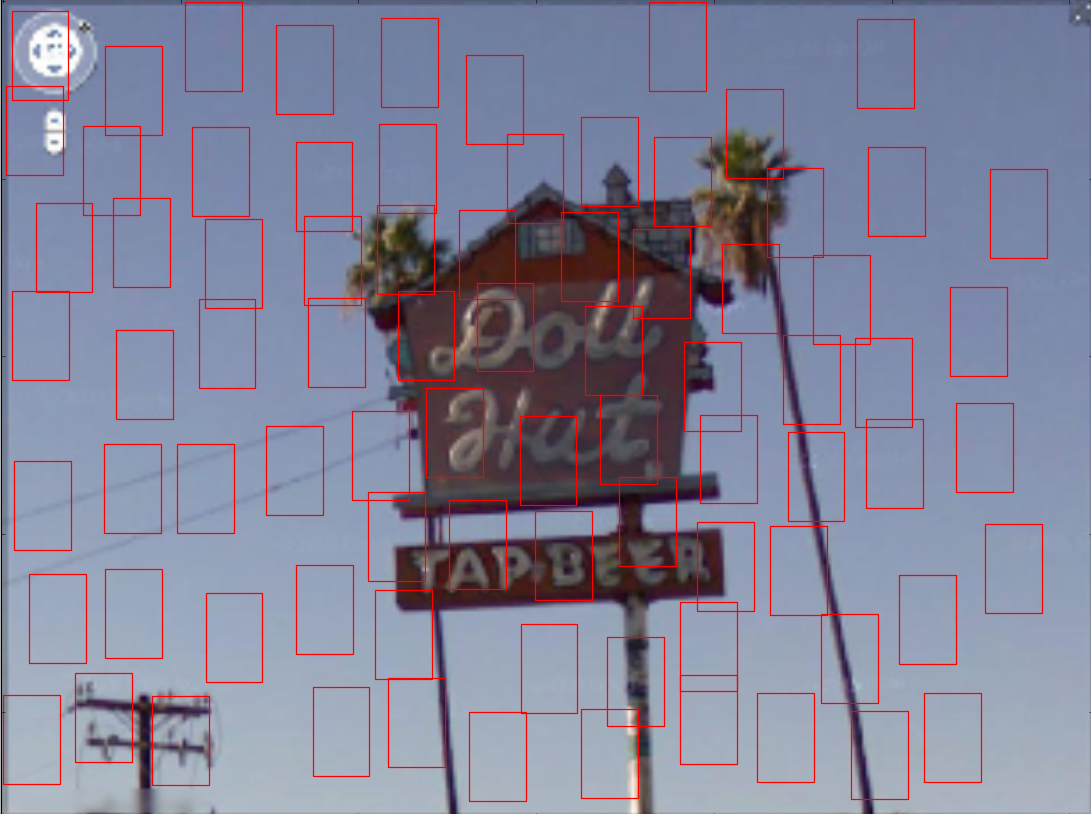
\includegraphics[width=0.3\columnwidth]{figures/beer2.png}
\caption{Spreading of the detected characters}
\end{figure}

\item The prior we use here is a bi-gram prior. It only take into account the succession of letter. One information we are not using is the fact that a 'P' is more frequent at the beginning of a word that at the end. We could thus follow the idea given in the paper \cite{Mis} to build a Node-specific prior. The idea is to compute for each graphical model a prior based on the place of the node in the image and in the graphical model. But this seems to be only possible after a cleaning of the graphical model in the first step. We should reduce the false positive rate and then extract all the connected components of our graph to build our lexical prior in this context.
\end{itemize}






\newpage

\bibliographystyle{unsrt}
\bibliography{biblio}





\end{document}